\documentclass{article}

\usepackage[a4paper,left=2.25cm,right=2.25cm,top=2.5cm,bottom=2.5cm]{geometry}

\title{Astable Multivibrator}
\author{David Roberts}
\date{}

\usepackage{tikz}
% (c) 2008 David Roberts

\usepackage{tikz}
\usetikzlibrary{arrows}

\tikzstyle{fliphorz} = [xscale=-1] % reflect left to right
\tikzstyle{flipvert} = [yscale=-1] % reflect top to bottom
\tikzstyle{component top} = []
\tikzstyle{component bottom} = []
\tikzstyle{component base} = []

\newcommand{\ohm}{\ensuremath{\Omega}}
\newcommand{\micro}{\ensuremath{\mu}}

\newcommand{\led}[2][]{
 \begin{scope}[shift={(#2)},#1]
  \begin{scope}[component top]
   \draw[opacity=1.0] (0,0) -- (0,-0.1);
   \filldraw[opacity=0.5,fill=white] (0.1,-0.1) -- (-0.1,-0.1) -- (0,-0.4) -- cycle;
   \draw[opacity=0.66,->,>=stealth] (0.15,-0.2) -- (0.25,-0.3);
   \draw[opacity=0.33,->,>=stealth] (0.15,-0.3) -- (0.25,-0.4);
   \draw[opacity=0.0] (0.1,-0.4) -- (-0.1,-0.4);
   \draw[opacity=0.0] (0,-0.4) -- (0,-0.5);
  \end{scope}
  \begin{scope}[component bottom]
   \draw[opacity=0.0] (0,0) -- (0,-0.1);
   \filldraw[opacity=0.5,fill=white] (0.1,-0.1) -- (-0.1,-0.1) -- (0,-0.4) -- cycle;
   \draw[opacity=0.33,->,>=stealth] (0.15,-0.2) -- (0.25,-0.3);
   \draw[opacity=0.66,->,>=stealth] (0.15,-0.3) -- (0.25,-0.4);
   \draw[opacity=1.0] (0.1,-0.4) -- (-0.1,-0.4);
   \draw[opacity=1.0] (0,-0.4) -- (0,-0.5);
  \end{scope}
 \end{scope}
}

\newcommand{\capacitor}[2][]{
 \begin{scope}[shift={(#2)},#1]
  \draw[component top] (0,0) -- (0,-0.45);
  \draw[component top] (0.15,-0.35) node {+};
  \draw[component top] (0.2,-0.45) -- (-0.2,-0.45);
  \draw[component bottom] (0.2,-0.55) -- (-0.2,-0.55);
  \draw[component bottom] (0,-0.55) -- (0,-1);
 \end{scope}
}

\newcommand{\transistor}[2][]{
 \begin{scope}[shift={(#2)},#1]
  \filldraw[fill=white] (-0.1,-0.5) circle (0.25);
  \draw[component top] (0,0) -- (0,-0.271); % C
  \draw[component top] (-0.25,-0.45) -- (0,-0.271); % BC
  \draw[component base] (-0.5,-0.5) -- (-0.25,-0.5); % B
  \draw[component base] (-0.25,-0.35) -- (-0.25,-0.65); % B plate
  \draw[component bottom,->,>=stealth] (-0.25,-0.55) -- (0,-0.729); % BE
  \draw[component bottom] (0,-0.729) -- (0,-1); % E
 \end{scope}
}

\newcommand{\crossover}[2][]{
 \begin{scope}[shift={(#2)},#1]
  \filldraw[white,fill=white] (0,0) circle (0.05);
  \draw (-0.05,0) arc (180:0:0.05);
 \end{scope}
}

\newcommand{\resistor}[2][]{
 \begin{scope}[shift={(#2)},#1]
  \begin{scope}[component top]
   \draw [opacity=1.0] (0,0) -- (0,-0.2);
   \draw [opacity=0.875] (0,-0.2) -- (0.1,-0.25);
   \draw [opacity=0.75] (0.1,-0.25) -- (-0.1,-0.35);
   \draw [opacity=0.625] (-0.1,-0.35) -- (0.1,-0.45);
   \draw [opacity=0.5] (0.1,-0.45) -- (-0.1,-0.55);
   \draw [opacity=0.375] (-0.1,-0.55) -- (0.1,-0.65);
   \draw [opacity=0.25] (0.1,-0.65) -- (-0.1,-0.75);
   \draw [opacity=0.125] (-0.1,-0.75) -- (0,-0.8);
   \draw [opacity=0.0] (0,-0.8) -- (0,-1);
  \end{scope}
  \begin{scope}[component bottom]
   \draw [opacity=0.0] (0,0) -- (0,-0.2);
   \draw [opacity=0.125] (0,-0.2) -- (0.1,-0.25);
   \draw [opacity=0.25] (0.1,-0.25) -- (-0.1,-0.35);
   \draw [opacity=0.375] (-0.1,-0.35) -- (0.1,-0.45);
   \draw [opacity=0.5] (0.1,-0.45) -- (-0.1,-0.55);
   \draw [opacity=0.625] (-0.1,-0.55) -- (0.1,-0.65);
   \draw [opacity=0.75] (0.1,-0.65) -- (-0.1,-0.75);
   \draw [opacity=0.875] (-0.1,-0.75) -- (0,-0.8);
   \draw [opacity=1.0] (0,-0.8) -- (0,-1);
  \end{scope}
 \end{scope}
}

\newcommand{\resistorbox}[2][]{
 \begin{scope}[shift={(#2)},#1]
  \draw[component top] (0,0) -- (0,-0.2);
  \filldraw[fill=white,opacity=0.5,component top]    (-0.1,-0.2) rectangle (0.1,-0.8);
  \draw[opacity=0.5,component bottom] (-0.1,-0.2) rectangle (0.1,-0.8);
  \draw[component bottom] (0,-0.8) -- (0,-1);
 \end{scope}
}

\newcommand{\vrail}[3][]{
 \begin{scope}[shift={(#3)},#1]
  \draw[o-] (0,0) node[left] {#2} -- (0.5,0);
 \end{scope}
}


\begin{document}
 \maketitle
 
 \begin{figure}[h!]
  \begin{center}
   \begin{tikzpicture}[scale=3.5]
    \vrail{9V}{-2,0}  \draw (-1.5,0) -- (1.5,0);
    \vrail{0V}{-2,-3} \draw (-1.5,-3) -- (1.5,-3);
    
    \resistor{-1.5,0}    \draw (-1.5,-0.5) node[left=8pt] {$R_1$} node[right=8pt] {390\ohm};
    \resistor{-0.5,-0.5} \draw (-0.5,-1)   node[left=8pt] {$R_2$} node[right=8pt] {22k\ohm};
     \draw (-0.5,0) -- (-0.5,-0.5);
     \draw (-0.5,-1.5) -- (-0.5,-2);
    \resistor{0.5,-0.5}  \draw (0.5,-1)    node[left=8pt] {$R_3$} node[right=8pt] {22k\ohm};
     \draw (0.5,0) -- (0.5,-0.5);
     \draw (0.5,-1.5) -- (0.5,-2);
    \resistor{1.5,0}     \draw (1.5,-0.5)  node[left=8pt] {$R_4$} node[right=8pt] {390\ohm};
    
    \led[fliphorz]{-1.5,-1} \draw (-1.5,-1.5) -- (-1.5,-2);
    \led{1.5,-1}            \draw (1.5,-1.5) -- (1.5,-2);
    
    \capacitor[rotate={90}]{-1.5,-2}          \draw (-1,-1.8) node[above] {$C_1$ 47\micro F};
    \capacitor[flipvert,rotate={270}]{1.5,-2} \draw (1,-1.8) node[above] {$C_2$ 47\micro F};
    
    \transistor[fliphorz]{-1.5,-2} \draw (-1.65,-2.5) node[left] {$Q_1$};
    \transistor{1.5,-2}            \draw (1.65,-2.5) node[right] {$Q_2$};
    
    % bases to capacitors
    \draw (-1,-2.5) -- (-0.5,-2.5) -- (0.5,-2); \crossover[rotate=22.5]{0,-2.25}
    \draw (1,-2.5) -- (0.5,-2.5) -- (-0.5,-2);
   \end{tikzpicture}
   \caption{Circuit Diagram}
  \end{center}
 \end{figure}
 
 \begin{figure}
  \begin{center}
   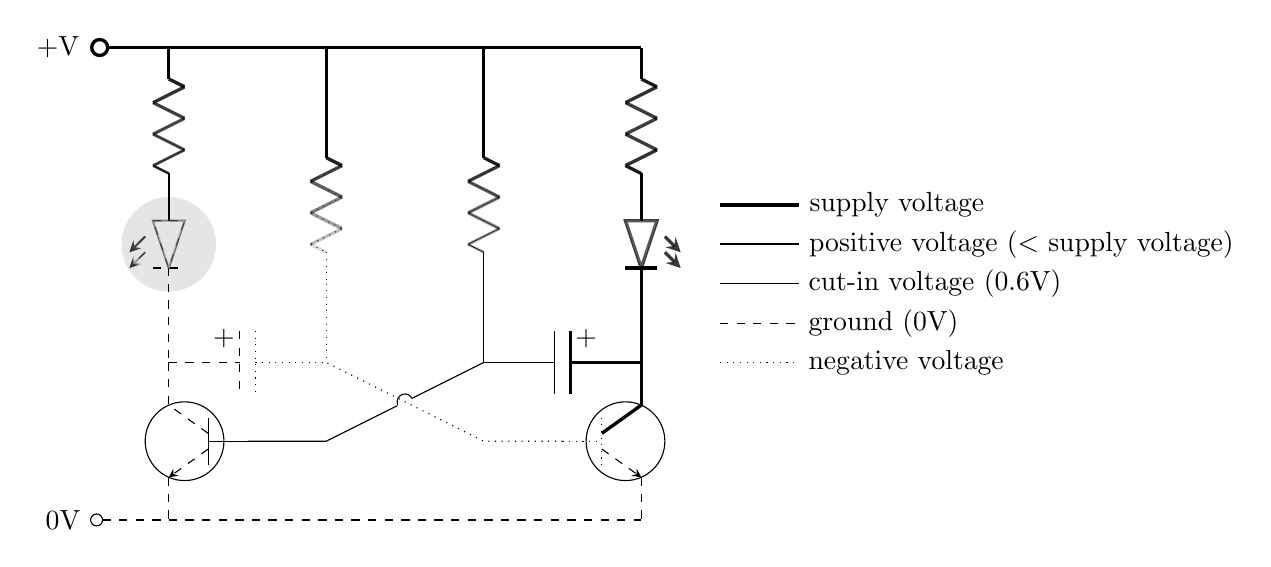
\begin{tikzpicture}[scale=2]
    \tikzstyle{voltpos} = [very thick]
    \tikzstyle{voltmedpos} = [thick]
    \tikzstyle{voltsmallpos} = []
    \tikzstyle{voltground} = [dashed]
    \tikzstyle{voltneg} = [dotted]
    
    \vrail[voltpos]{+V}{-2,0}     \draw[voltpos] (-1.5,0) -- (1.5,0);
    \vrail[voltground]{0V}{-2,-3} \draw[voltground] (-1.5,-3) -- (1.5,-3);
    
    \tikzstyle{component top} = [voltpos] \tikzstyle{component bottom} = [voltmedpos]
     \resistor{-1.5,0}
    \tikzstyle{component top} = [voltpos] \tikzstyle{component bottom} = [voltneg]
     \resistor{-0.5,-0.5}
     \draw[voltpos] (-0.5,0) -- (-0.5,-0.5);
     \draw[voltneg] (-0.5,-1.5) -- (-0.5,-2);
    \tikzstyle{component top} = [voltpos] \tikzstyle{component bottom} = [voltsmallpos]
     \resistor{0.5,-0.5}
     \draw[voltpos] (0.5,0) -- (0.5,-0.5);
     \draw[voltsmallpos] (0.5,-1.5) -- (0.5,-2);
    \tikzstyle{component top} = [voltpos] \tikzstyle{component bottom} = [voltpos]
     \resistor{1.5,0}
    
    \tikzstyle{component top} = [voltmedpos] \tikzstyle{component bottom} = [voltground]
     \led[fliphorz]{-1.5,-1}
     \draw[voltground] (-1.5,-1.5) -- (-1.5,-2);
     \fill[black,opacity=0.1] (-1.5,-1.25) circle (0.3);
    \tikzstyle{component top} = [voltpos]    \tikzstyle{component bottom} = [voltpos]
     \led{1.5,-1}
     \draw[voltpos] (1.5,-1.5) -- (1.5,-2);
    
    \tikzstyle{component top} = [voltground] \tikzstyle{component bottom} = [voltneg]
     \capacitor[rotate={90}]{-1.5,-2}
    \tikzstyle{component top} = [voltpos]    \tikzstyle{component bottom} = [voltsmallpos]
     \capacitor[flipvert,rotate={270}]{1.5,-2}
    
    \tikzstyle{component top} = [voltground] \tikzstyle{component bottom} = [voltground] \tikzstyle{component base} = [voltsmallpos]
     \transistor[fliphorz]{-1.5,-2}
    \tikzstyle{component top} = [voltpos]    \tikzstyle{component bottom} = [voltground] \tikzstyle{component base} = [voltneg]
     \transistor{1.5,-2}
    
    % bases to capacitors
    \draw[voltsmallpos] (-1,-2.5) -- (-0.5,-2.5) -- (0.5,-2); \crossover[voltsmallpos,rotate={22.5}]{0,-2.25}
    \draw[voltneg] (1,-2.5) -- (0.5,-2.5) -- (-0.5,-2);
    
    % legend
    \begin{scope}[shift={(2,-1)}]
     \draw[voltpos]      (0,0) -- (0.5,0)   node[right] {supply voltage};
     \draw[voltmedpos]   (0,-0.25) -- (0.5,-0.25) node[right] {positive voltage ($<$ supply voltage)};
     \draw[voltsmallpos] (0,-0.5) -- (0.5,-0.5) node[right] {cut-in voltage (0.6V)};
     \draw[voltground]   (0,-0.75) -- (0.5,-0.75) node[right] {ground (0V)};
     \draw[voltneg]      (0,-1) -- (0.5,-1) node[right] {negative voltage};
    \end{scope}
   \end{tikzpicture}
   \caption{Voltages --- Greyscale}
  \end{center}
 \end{figure}
 
 \begin{figure}
  \begin{center}
   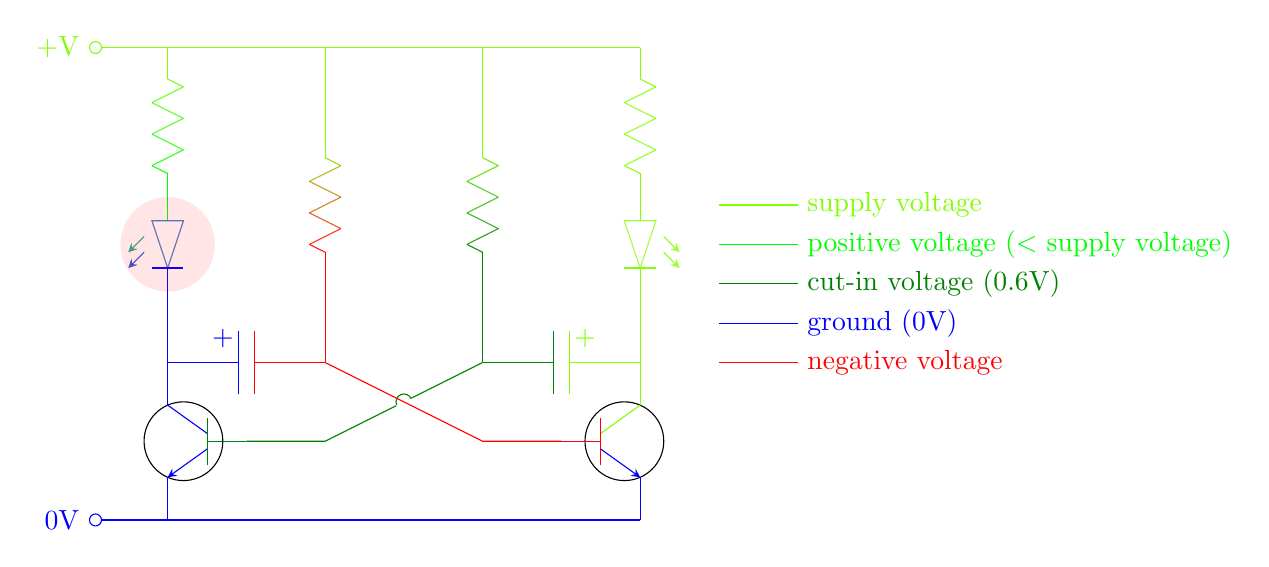
\begin{tikzpicture}[scale=2]
    \tikzstyle{voltpos} = [green!50!yellow]
    \tikzstyle{voltsmallpos} = [green!50!black]
    \tikzstyle{voltmedpos} = [green]
    \tikzstyle{voltneg} = [red]
    \tikzstyle{voltground} = [blue]
    
    \vrail[voltpos]{+V}{-2,0}     \draw[voltpos] (-1.5,0) -- (1.5,0);
    \vrail[voltground]{0V}{-2,-3} \draw[voltground] (-1.5,-3) -- (1.5,-3);
    
    \tikzstyle{component top} = [voltpos] \tikzstyle{component bottom} = [voltmedpos]
     \resistor{-1.5,0}
    \tikzstyle{component top} = [voltpos] \tikzstyle{component bottom} = [voltneg]
     \resistor{-0.5,-0.5}
     \draw[voltpos] (-0.5,0) -- (-0.5,-0.5);
     \draw[voltneg] (-0.5,-1.5) -- (-0.5,-2);
    \tikzstyle{component top} = [voltpos] \tikzstyle{component bottom} = [voltsmallpos]
     \resistor{0.5,-0.5}
     \draw[voltpos] (0.5,0) -- (0.5,-0.5);
     \draw[voltsmallpos] (0.5,-1.5) -- (0.5,-2);
    \tikzstyle{component top} = [voltpos] \tikzstyle{component bottom} = [voltpos]
     \resistor{1.5,0}
    
    \tikzstyle{component top} = [voltmedpos] \tikzstyle{component bottom} = [voltground]
     \led[fliphorz]{-1.5,-1}
     \draw[voltground] (-1.5,-1.5) -- (-1.5,-2);
     \fill[red,opacity=0.1] (-1.5,-1.25) circle (0.3);
    \tikzstyle{component top} = [voltpos]    \tikzstyle{component bottom} = [voltpos]
     \led{1.5,-1}
     \draw[voltpos] (1.5,-1.5) -- (1.5,-2);
    
    \tikzstyle{component top} = [voltground] \tikzstyle{component bottom} = [voltneg]
     \capacitor[rotate={90}]{-1.5,-2}
    \tikzstyle{component top} = [voltpos]    \tikzstyle{component bottom} = [voltsmallpos]
     \capacitor[flipvert,rotate={270}]{1.5,-2}
    
    \tikzstyle{component top} = [voltground] \tikzstyle{component bottom} = [voltground] \tikzstyle{component base} = [voltsmallpos]
     \transistor[fliphorz]{-1.5,-2}
    \tikzstyle{component top} = [voltpos]    \tikzstyle{component bottom} = [voltground] \tikzstyle{component base} = [voltneg]
     \transistor{1.5,-2}
    
    % bases to capacitors
    \draw[voltsmallpos] (-1,-2.5) -- (-0.5,-2.5) -- (0.5,-2); \crossover[voltsmallpos,rotate={22.5}]{0,-2.25}
    \draw[voltneg] (1,-2.5) -- (0.5,-2.5) -- (-0.5,-2);
    
    % legend
    \begin{scope}[shift={(2,-1)}]
     \draw[voltpos]      (0,0) -- (0.5,0)   node[right] {supply voltage};
     \draw[voltmedpos]   (0,-0.25) -- (0.5,-0.25) node[right] {positive voltage ($<$ supply voltage)};
     \draw[voltsmallpos] (0,-0.5) -- (0.5,-0.5) node[right] {cut-in voltage (0.6V)};
     \draw[voltground]   (0,-0.75) -- (0.5,-0.75) node[right] {ground (0V)};
     \draw[voltneg]      (0,-1) -- (0.5,-1) node[right] {negative voltage};
    \end{scope}
   \end{tikzpicture}
   \caption{Voltages --- Colour}
  \end{center}
 \end{figure}
\end{document}
